\documentclass{article}

\usepackage{ctex}
\usepackage{graphicx}
\usepackage{amsmath, bm}
\usepackage{url}
\newtheorem{exmp}{Example}

\title{MIT18.02 Multivariable Calculus}
\author{Xingdong Xue}
\date{Dec. 2019}

\newcommand\printvec[1]{\mathbf{#1}}
\newcommand\norm[1]{\mathbf{\left| \printvec{#1} \right|}}
\newcommand\lrangle[1]{\left \langle #1 \right \rangle}
\newcommand\directv{\hat{\mathbf{u}}}
\newcommand\deter[1]{\left| #1 \right|}

\begin{document}
\maketitle

\section{Vectors and Matrices}
\subsection{Vectors}
A vector can be viewd in to different ways: geometrically and algebraically.

\textbf{Geometric view}

A vector is defined as having a magnitude and a direction, the start of the arrow is tail, and the end is denoted as the tip or head.
\begin{figure}[htbp]
  \centering
  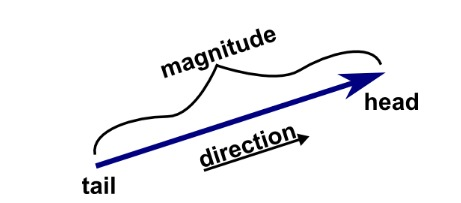
\includegraphics[width=.8\textwidth]{vector.jpg}
  \caption{vector}
  \label{vector}
\end{figure}

The vector between two points will be denoted $\overrightarrow{PQ}$. $P$ is the initial point and $Q$ is the terminal point.

The magnitude of the vector \textbf{A} will be denoted $\mathbf{\left| A \right|}$. Magnitude will also be called \textit{length} or \textit{norm}.

\textbf{Scaling, adding and subtracting vectors}

\begin{enumerate}
  \item Scaling: Scaling a vector means changing its length by a scale factor. Because we use numbers to scale a vector we will often refer to real numbers as \textit{scalars}.
  \item Add: Add vectors by placing them head to tail, this can be done in either order.
  \item Substract: Subtract vectors either by placing the tail to tail or by adding $\mathbf{A+(-B)}$.
\end{enumerate}

\textbf{Algebra view}

The origin is labeld as $O$, $O = (0, 0)$ in the plane and $O = (0, 0, 0)$ in the space.
If the tail of the vector is placed at origin, we call it \textit{origin vector} and the vector is denoted $A = \lrangle{a_1, a_2}$.

We can do calculation by using two vectors $\mathbf{i} = \lrangle{1, 0}$, $\mathbf{j} = \lrangle{0, 1}$

\textbf{Notations and terminology}

\begin{enumerate}
  \item $(a_1, a_2)$ indicates a point in the plane.
  \item $\lrangle{a_1, a_2} = a_1\mathbf{i} + a_2\mathbf{j}$.
  \item for $\mathbf{A} = \lrangle{a_1, a_2} = a_1\mathbf{i} + a_2\mathbf{j}$, $a_1$ and $a_2$ is called the $\mathbf{i}$ and $\mathbf{j}$ components of $\mathbf{A}$.
  \item $\overrightarrow{P} = \overrightarrow{OP}$ is the vector from the origin to $P$.
  \item A real number is a $\textit{scalar}$, you can use it to scale a vector.
\end{enumerate}

\textbf{Vector algebra using coordinates}

\begin{enumerate}
  \item Magnitude: $\norm{A} = \sqrt{a_1^2+a_2^2}$.
  \item Addition/Substraction: $\mathbf{A \pm B} = (a_1 \pm b_1)\mathbf{i} + (a_2 \pm b_2)\mathbf{j}$.
  \item $\overrightarrow{PQ} = \overrightarrow{Q} - \overrightarrow{P}$, $\overrightarrow{PQ}$ is the $\textit{displacement}$ from $P$ to $Q$.
  \item in three dimensions, $\norm{A} = \sqrt{a_1^2+a_2^2+a_3^2}$.
\end{enumerate}

\textbf{Unit vectors}

A unit vector is a vector with unit length. It's denoted $\directv$.

\subsection{Dot product}

Dot product is a way of multipling two vectors. It's also called \textit{scalar product} because the result of it is a scalar.

\textbf{Algebraic definition}
if $\printvec{A} = \lrangle{a_1, a_2}$ and $\printvec{B} = \lrangle{b_1, b_2}$ then
$$\printvec{A} \cdot \printvec{B} = a_1b_1 + a_2b_2$$

\textbf{Geometric definition}
$$\printvec{A} \cdot \printvec{B} = \norm{A}\norm{B}\cos\theta$$
$$\norm{A - B}^2 = \norm{A}^2 + \norm{B}^2 - 2\norm{A}\norm{B}\cos\theta$$
$$\printvec{A} \cdot (\printvec{B} + \printvec{C}) = \printvec{A} \cdot \printvec{B} + \printvec{A} \cdot \printvec{C}$$
When two vectors are perpendicular to each other we say they are \textit{orthogonal}. $\printvec{A} \perp \printvec{B} \Leftrightarrow \printvec{A} \cdot \printvec{B} = 0$

\textbf{Dot product and length}

Algebraically: $\printvec{A} \cdot \printvec{A} = \lrangle{a_1, a_2, a_3} \cdot \lrangle{a_1, a_2, a_3} = \norm{A}^2$

Geometrically: $\printvec{A} \cdot \printvec{A} = \norm{A}\norm{A}\cos\theta = \norm{A}\norm{A} = \norm{A}^2$

\subsection{Uses of dot product}
\begin{enumerate}
  \item Find the angle between two vectors(either in a plane or space).
  \item Judge if two vectors are orthogonal.
  \item Using vectors and dot product show the diagonals of a parallelogram have equal lengths
        if and only if it’s a rectangle.
  \item Dot product shows the degree of collinearity, if there is a right-handed coordinate system $\printvec{i}^\prime$ and $\printvec{j}^\prime$.
        To express vector $\printvec{A}$ in this coordinate system, the coordinate of $\printvec{A}^\prime$ is $\lrangle{\printvec{A} \cdot \printvec{i}^\prime, \printvec{A} \cdot \printvec{j}^\prime}$.
\end{enumerate}

\subsection{Components and Projection}
If $\printvec{A}$ is any vector and $\directv$ is a unit vector then the component of $\printvec{A}$ in the direction of $\directv$ is
$$\printvec{A} \cdot \directv.$$

And if $\theta$ is the angle between $\printvec{A}$ and $\directv$, then
$$\printvec{A} \cdot \directv = \printvec{A}\cos\theta$$
We also call the leg parallel to $\directv$ the \textit{orthogonal projection} of $\mathbf{A}$ on $\directv$.

\subsection{Areas and Determinants}

The value of the determinant is area of the parallelogram formed by $\mathbf{A}$ and $\mathbf{B}$.
$\mathbf{A} = \lrangle{a_1, b_1}$, $\mathbf{B} = \lrangle{a_2, b_2}$.
\begin{equation*}
  \det(\mathbf{A}, \mathbf{B})
  = \begin{vmatrix}
    a_1 & a_2 \\
    b_1 & b_2 \\
  \end{vmatrix}
  = a_1b_2 - a_2b_1
\end{equation*}


\subsection{Determinant in space}

\textbf{Important facts about $\deter{A}$}
\begin{enumerate}
  \item $\deter{A}$ is multiplied by −1 if we interchange two rows or two columns.
  \item $\deter{A} = 0$ if one row or column is all zero, or if two rows or two columns are the same.
  \item $\deter{A}$ is multiplied by $c$, if every element of some row or column is multiplied by $c$.
  \item The value of $\deter{A}$ is unchanged if we add to one row (or column) a constant multiple of another row (resp. column).
\end{enumerate}

The $\mathbf{ij}$-$\textbf{entry}$, written $a_{ij}$, is the number in the $i$-th row and $j$-th column. \\
The $\mathbf{ij}$-$\textbf{minor}$, written $\left| A_{ij} \right|$, is the determinant that’s left after deleting from $\deter{A}$ row
and column containing $a_{ij}$. \\
The $\mathbf{ij}$-$\textbf{cofactor}$, written $A_{ij}$, is given as a formula by $A_{ij} = (−1)^{i+j}\left| A_{ij} \right|$.

\textbf{Laplace expansion by cofactors}
$$a_{1j}A_{1j} + a_{2j}A_{2j} + a_{3j}A_{3j} = \deter{A}$$

\subsection{Cross Product}

Cross product is another way of multiplying two vectors. Because the result of this multiplication is another
vector it is also called the \textit{vector product}.

$\mathbf{A} = \lrangle{a_1, a_2, a_3}$, $\mathbf{B} = \lrangle{b_1, b_2, b_3}$
\begin{equation*}
  \mathbf{A} \times \mathbf{B}
  = \begin{vmatrix}
    \mathbf{i} & \mathbf{j} & \mathbf{k} \\
    a_1        & a_2        & a_3        \\
    b_1        & b_2        & b_3
  \end{vmatrix}
  = \lrangle{a_2b_3 - a_3b_2, a_3b_1 - a_1b_3, a_1b_2 - a_2b_1}
\end{equation*}

\textbf{Algebraic facts}
\begin{enumerate}
  \item $\mathbf{A} \times \mathbf{A} = 0$
  \item Anti-commutivity: $\mathbf{A} \times \mathbf{B} = -\mathbf{B} \times \mathbf{A}$
  \item Distributive law: $\mathbf{A} \times (\mathbf{B}+\mathbf{C}) =  \mathbf{A} \times \mathbf{B} + \mathbf{A} \times \mathbf{C}$
  \item Non-associativity: $(\mathbf{A} \times \mathbf{B}) \times \mathbf{C} \neq \mathbf{A} \times (\mathbf{B} \times \mathbf{C})$
\end{enumerate}

$$\mathbf{i} \times \mathbf{j} = \mathbf{k}, \mathbf{j} \times \mathbf{k} = \mathbf{i}, \mathbf{k} \times \mathbf{i} = \mathbf{j}$$

\textbf{Geometric description}
$\deter{\mathbf{A} \times \mathbf{B}} = \norm{A}\norm{B}\sin\theta$, it is also the area of the parallelogram spanned by $\mathbf{A}$ and $\mathbf{B}$.

The direction of $\deter{\mathbf{A} \times \mathbf{B}}$ is determined by \textit{right hand rule}.

\subsection{Equation of a Plane}

Judging if point $P(x, y, z)$ is in the plane which points $P_1$, $P_2$ and $P_3$ are in is equal to judging if $\overrightarrow{P_1P} \cdot (\overrightarrow{P_1P_2} \times \overrightarrow{P_1P_3}) = 0$.
$$V = \left[ a, b, c \right] = a \cdot (b \times c) = b \cdot (c \times a) = c \cdot (a \times b) = det(a, b, c)$$
So it's equal to $det(\overrightarrow{P_1P}, \overrightarrow{P_1P_2}, \overrightarrow{P_1P_3}) = 0$

\subsection{Matrix Algebra}
\textbf{Matrix algebra}

A rectangular array of numbers having $n$ rows and $n$ columns is called an $m × n$ \textbf{matrix}.

Two matrices of the same size are \textit{equal} if corresponding entries are equal.

Two special kinds of matrices are the \textbf{row-vectors}: the $1 \times n$ matrices; and the \textbf{column vectors}: the $m \times 1$ matrices consisting of a column of $m$ numbers.

\textbf{Matrix operations}
\begin{enumerate}
  \item Scalar multiplication
  \item Matrix addition
  \item Transposition
  \item Matrix multiplication
\end{enumerate}

\textbf{Laws and properties of matrix multiplication}
\begin{enumerate}
  \item $A(B+C) = AB + AC \quad (A + B)C = AC + BC \quad \textit{distributive laws}$
  \item $(AB)C = A(BC) \quad (cA)B = c(AB)  \textit{associative laws}$
  \item $I_3 =  \begin{vmatrix}
            1 & 0 & 0 \\
            0 & 1 & 0 \\
            0 & 0 & 1 \\
          \end{vmatrix}$
  \item In general, $AB \neq BA$,
  \item $\deter{AB} = \deter{A}\deter{B}$
  \item Matrix multiplication can be used to pick out a row or column of a given matrix, such as
        $$
          \begin{pmatrix}
            1 & 0 & 0
          \end{pmatrix}
          \begin{pmatrix}
            1 & 2 & 3 \\
            4 & 5 & 6 \\
            7 & 8 & 9 \\
          \end{pmatrix}
          =
          \begin{pmatrix}
            1 & 2 & 3
          \end{pmatrix}
        $$
        $$
          \begin{pmatrix}
            1 & 2 & 3 \\
            4 & 5 & 6 \\
            7 & 8 & 9 \\
          \end{pmatrix}
          \begin{pmatrix}
            0 \\
            1 \\
            0
          \end{pmatrix}
          =
          \begin{pmatrix}
            2 \\
            5 \\
            8
          \end{pmatrix}
        $$
\end{enumerate}

\subsection{Meaning of matrix multiplication}
Matrix transforms the unit square into a parallelogram.
$$A =
  \begin{pmatrix}
    4 & 1 \\
    2 & 3
  \end{pmatrix}
$$
$$A\textbf{i} = A
  \begin{pmatrix}
    1 \\
    0
  \end{pmatrix} =
  \begin{pmatrix}
    4 \\
    1
  \end{pmatrix};\quad
  A\textbf{j} = A
  \begin{pmatrix}
    0 \\
    1
  \end{pmatrix} =
  \begin{pmatrix}
    1 \\
    3
  \end{pmatrix}
$$

\begin{figure}[htbp]
  \centering
  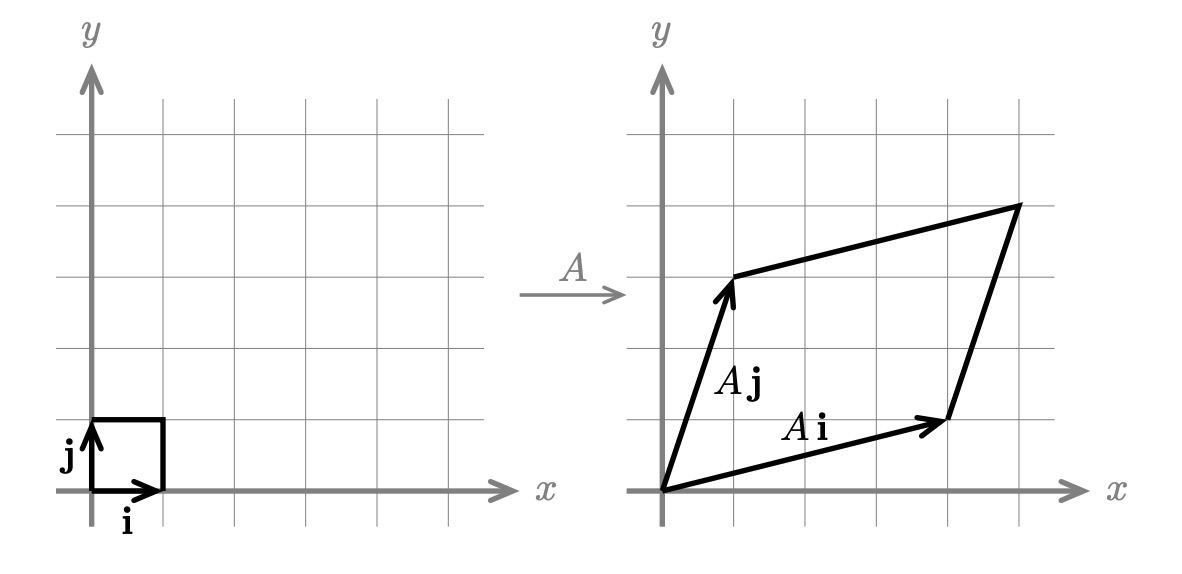
\includegraphics[width=.8\textwidth]{matrix_multiplication.png}
  \caption{vector}
  \label{vector}
\end{figure}

\subsection{Solving Square Systems of Linear Equations; Inverse Matrices}
\begin{gather*}
  MA = I \\
  A\textbf{x} = \textbf{b} \\
  M(A\textbf{x}) = M\textbf{b} \\
  \textbf{x} = M\textbf{b}
\end{gather*}

We can solve $\textbf{y} = M\textbf{x}$ by solving $\textbf{x} = A\textbf{y}$ where $A$ is the inverse matrix of $M$.

\textbf{Inverse Matrices}

Let A be an $n \times n$ matrix, with $\deter{A} \neq 0$. Then the inverse of A is an $n \times n$
matrix, written $A^{-1}$.
$$A^{-1}A = I_n$$

$$A^{-1} = \frac{1}{\deter{A}}adj A = \frac{1}{\deter{A}}
  \begin{pmatrix}
    A_{11} & A_{12} & A_{13} \\
    A_{21} & A_{22} & A_{23} \\
    A_{31} & A_{32} & A_{33} \\
  \end{pmatrix}^T
$$

where $A_{ij}$ is the cofactor of the element $a_{ij}$.

\subsection{Equations of Planes II}
\textbf{Planes in point-normal form}

If $\mathbf{N}$ is orthogonal to the plane, we call $\mathbf{N}$ the \textit{normal} vector of the plane.
And if $P_0$ is on the plane, then the equation of the plane would be:
\begin{align*}
   & \textbf{N} \cdot \overrightarrow{P_0P} = 0                                \\
   & \Leftrightarrow \lrangle{a, b, c} \cdot \lrangle{x-x_0, y-y_0, z-z_0} = 0 \\
   & \Leftrightarrow a(x−x_0) + b(y−y_0) + c(z−z_0) = 0
\end{align*}
\begin{exmp}
  Find the plane containing the points $P1 = (1, 2, 3)$, $P2 = (0, 0, 3)$, $P3 = (2, 5, 5)$.
  \begin{align*}
    \mathbf{N} = \overrightarrow{\mathbf{P_1P_2}} \times \overrightarrow{\mathbf{P_1P_3}}
    = \begin{pmatrix}
      \mathbf{i} & \mathbf{j} & \mathbf{k} \\
      -1         & 2          & 0          \\
      1          & 3          & 2
    \end{pmatrix}
    = −4\mathbf{i} − \mathbf{j}(−2) + \mathbf{k}(−1) = \lrangle{-4,2,1}
  \end{align*}
\end{exmp}

\subsection{Geometry of linear systems of equations}

The geometric picture makes this obvious. Here are the three possibilities.
\begin{enumerate}
  \item The two lines intersect in a point, so there is one solution.
  \item The two lines are parallel (and not the same), so there are no solutions.
  \item The two lines are the same, so there are an infinite number of solutions.
\end{enumerate}

\textbf{3 $\times$ 3 systems}
\begin{enumerate}
  \item Intersect in a point (1 solution to system).
  \item Intersect in a line ($\infty$ solutions).
        \begin{enumerate}
          \item Three different planes, the third plane contains the line of intersection of the first two.
          \item Two planes are the same, the third plane intersects them in a line.
        \end{enumerate}
  \item Intersect in a plane ($\infty$ solutions)
        \begin{enumerate}
          \item All three planes are the same.
        \end{enumerate}
  \item The planes don’t all intersect at any point (0 solutions).
        \begin{enumerate}
          \item The planes are different, but all parallel.
          \item Two planes are parallel, the third crosses them.
          \item The planes are different and none are parallel. but the lines of intersection of each pair are parallel.
          \item Two planes are the same and parallel to the third.
        \end{enumerate}
\end{enumerate}

\subsection{Solutions to linear systems}

\subsection{Parametric equations of lines}
\textbf{General parametric equations}
Given a point $(x, y, z)$, Thinking the position of the point depends on $t$ we written
$$x = x(t), y = y(t), z = z(t)$$
We call t the parameter and the equations for $x$, $y$ and $z$ are called \textit{parametric equations}.

\textbf{Parametric equations of lines}
In general, the line through $P_0 = (x_0, y_0, z_0)$ in the direction of $\printvec{v}\lrangle{v_1, v_2, v_3}$ has parametrization
$$\lrangle{x, y, z} = \lrangle{x_0+tv_1, y_0 + tv_2, z_0 + tv_3}$$

\subsection{Intersection of a line and a plane}
To find all points of intersection of $P$ with the line, we substitute the formulas for $x$, $y$ and $z$ into the equation for $P$ and solve for $t$.

\subsection{Parametric Curves}

\end{document}